\chapter{Лекция}
\label{ch:intro}

\section*{\textbf{Введение}}

На прошлом занятии мы познакомились с двумя типами модуляции: BPSK и QPSK и программно реализовали их. При реализации логики
PSF нужно было формировать прямоугольный импульс. Я сделал это самым простым методом: увеличивал кол-во значений I и Q. За счёт этого
получали I(t) и Q(t), которые уже длились во времени. Данный подход рабочий и не является ошибкой, но на практике не используется,
поскольку подходит только в случае, когда формирующий фильтр имеет прямоугольную импульсную характеристику. Если импульсная характеристика
имеет форму приподнятого косинуса, то такой метод не сработает. На этом занятии изучим более граммотный подход.


\section*{\textbf{Почему форма символов так важна?}}
Форма передаваемых символлов $I_n(t), Q_n(t)$ определяет свойства спектра радиосигнала. Если форма символов прямоугольная, то форма
спектра будет иметь вид функции $\frac{sinx}{x}$ и будет занимать большую ширину спектра. В реальных системах чаще всего используется форма приподнятого косинуса.

\section*{\textbf{Upsampling}}

Итак, мы хотим, чтобы I и Q были не просто числами, а имели длительность, т.е хотим получить I(t) и Q(t). 
Необходимо установить число семплов, которое будут длиться I и Q. Введем параметр L, который измеряется в $\frac{sample}{symbol}$
и будет отвечать за кол-во семплов, приходящихся на 1 символ, т.е за длительность символа. Если мы хотим сделать символы длящимися,
то необходимо поднять частоту дискретизации. Для этого существуют специальные блоки, которые называются Upsampling блоками. Их задача
состоит в увеличении частоты дискретизации. Во сколько раз нужно увеличить частоту дискретизации? Если на каждый символ теперь
приходится L семплов, то и частота дискретизации должна стать в L раз больше. За частоту дискретизации отвечает параметр $f_symb$ (символьная скорость),
который показывает скорость, с которой символы поступают из маппера. Соответсвенно после выхода из Upsampling блока получим
$f_s = f_{symb} * L$, т.е кол-во семплов на секунду времени (sample\_rate). Исходя из этого можно определить расстояние во времени
между семплами $T_s = \frac{1}{f_s}$.

\begin{figure}[H]
    \centering
    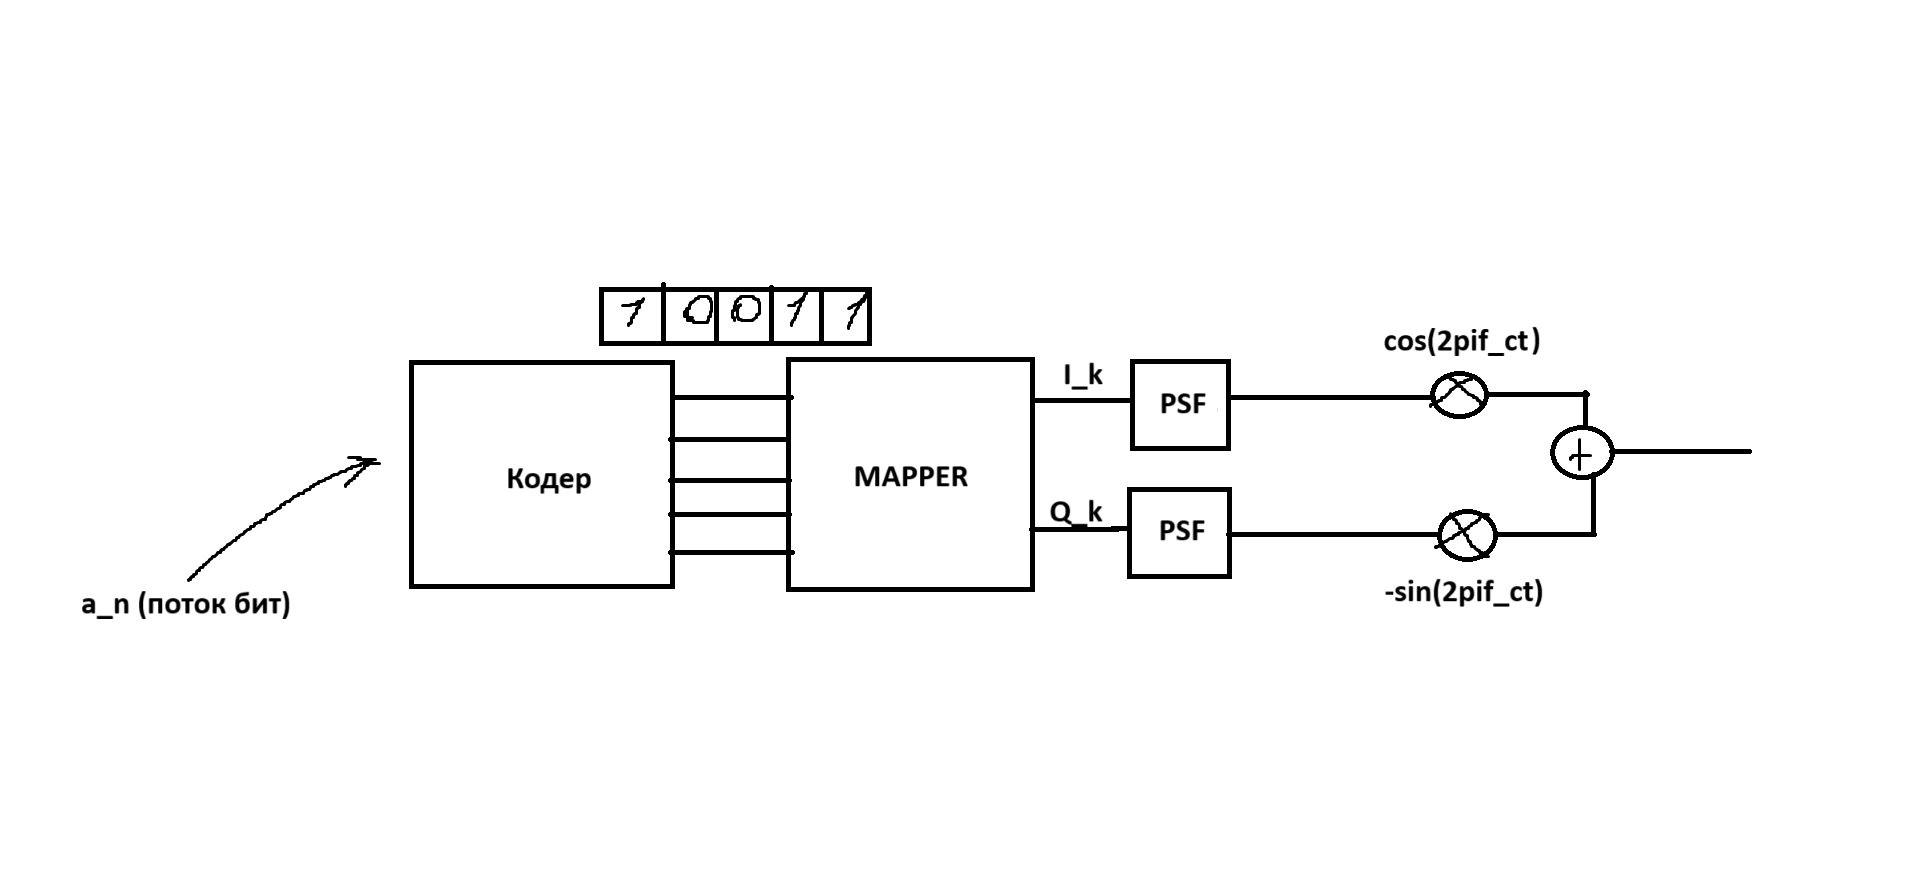
\includegraphics[width=1.0\textwidth]{tx_arch.png}
    \caption{Визуализация архитектуры передатчика}
\end{figure}

\section*{\textbf{Техническая реализация Upsampling}}

Техническую реализацию проще будет показать на примере. \\

Пусть на выходе маппера мы получили $I$ = [1, -1, 1], и хотим, чтобы каждый символ длился L = 4 семпла\\

Сформируем новую последовательность X(n), в которой между каждым $I_n$ добавим L-1 нулей.

\begin{figure}[H]
    \centering
    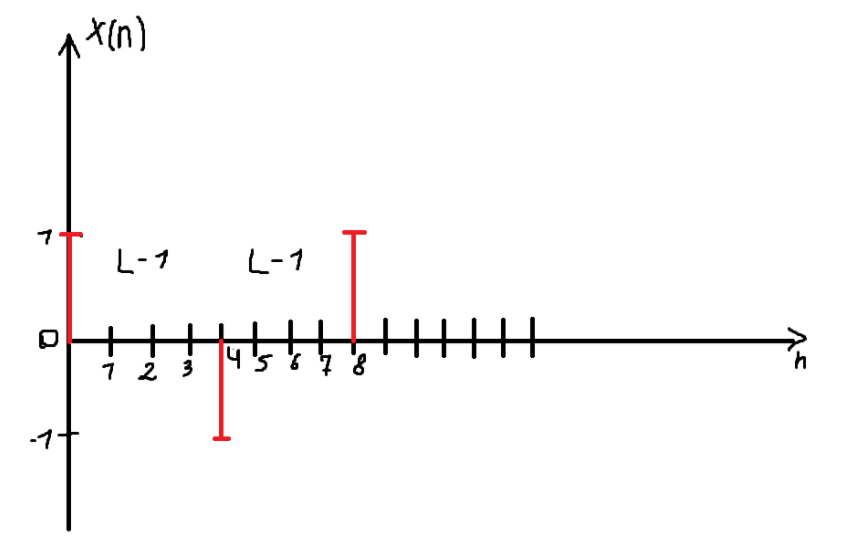
\includegraphics[width=1.0\textwidth]{Xn.png}
    \caption{Визуализация работы Upsampling}
\end{figure}

Получаем последовательность длинной 12 отсчетов (после последнего символа тоже идет 3 нуля).

\section*{\textbf{Формирующий фильтр}}

На данный момент мы только "растянули" символы, но не придали им никакой формы. Эти действия выполняет формирующий фильтр (на схеме g(n)). \\

В блоке g(n) происходят следующие расчеты: S(n) = $\sum_{m = 0}^{L-1}X(m)g(n-m)$, где X(n) - отсчеты, g(n) - импульсная характеристика фильтра.
Сама формула это дискретная свертка. \\

Импульсная характеристика фильтра имеет сложную форму, которая позволяет сделать сигнал любой формы. \\

Зададим форму импульсной характеристики. Для упрощения возьмем прямоугольную форму.

\begin{figure}[H]
    \centering
    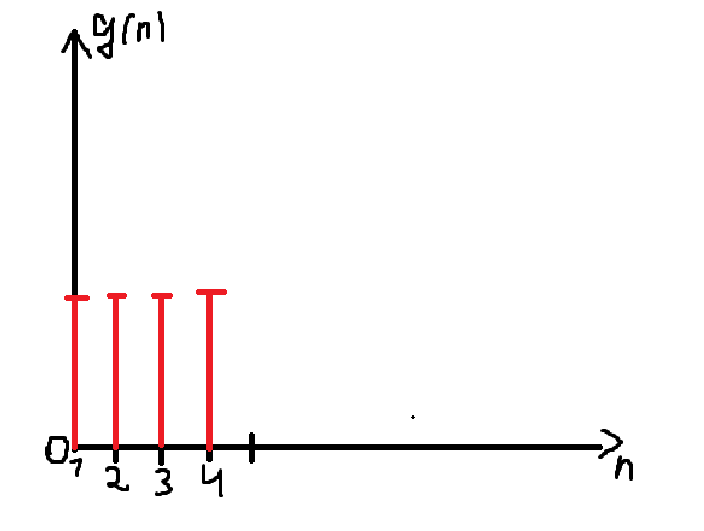
\includegraphics[width=1.0\textwidth]{gn.png}
    \caption{Пример импульсной характеристики}
\end{figure}

Для иллюстрации работы фильтра произведем вычисления по формуле выше:\\

S(0) = X(0)g(0) = 1*1 = 1\\

S(1) = X(0)g(1) + X(1)g(0) = 1*1 + 0*1 = 1 \\

S(2) = X(0)g(2) + X(1)g(1) + X(2)g(0) = 1*1 + 0*1 + 0*1 = 1 \\

S(3) = X(0)g(3) + X(1)g(2) + X(2)g(1) + X(3)g(0) = 1*1 + 0*1 + 0*1 + 0*1 = 1\\

S(4) = X(0)g(4) + X(1)g(3) + X(2)g(2) + X(3)g(1) + X(4)g(0) = 1*0 + 0*1 + 0*1 + 0*1 + (-1 * 1) = -1\\

S(4) = X(0)g(5) + X(1)g(4) + X(2)g(3) + X(3)g(2) + X(4)g(1) + X(5)g(0) = 1*0 + 0*0 + 0*1 + 0*1 + (-1 * 1) + 0 * 1 = -1\\

Визуализируем символы после выхода из фильтра:

\begin{figure}[H]
    \centering
    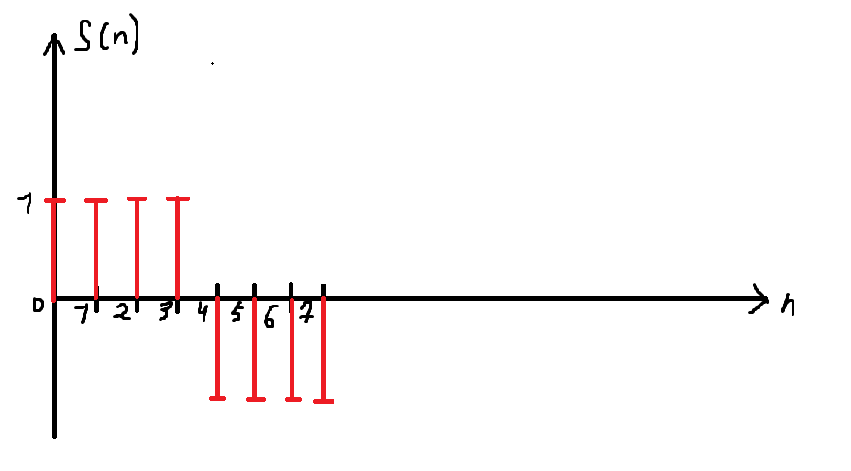
\includegraphics[width=1.0\textwidth]{sn.png}
    \caption{Пример символов после выхода из фильтра}
\end{figure}

Получили растянутые во времени I и Q с прямоугольной формой. Таким образом можно задать сигналу любую форму.

\endinput

